% This is samplepaper.tex, a sample chapter demonstrating the
% LLNCS macro package for Springer Computer Science proceedings;
% Version 2.21 of 2022/01/12
%
\documentclass[runningheads]{llncs}
%
\usepackage[T1]{fontenc}
% T1 fonts will be used to generate the final print and online PDFs,
% so please use T1 fonts in your manuscript whenever possible.
% Other font encondings may result in incorrect characters.
%
\usepackage{amsmath}
\usepackage{graphicx}
\usepackage{algorithm}
\usepackage{algpseudocode}
% Used for displaying a sample figure. If possible, figure files should
% be included in EPS format.
%
% If you use the hyperref package, please uncomment the following two lines
% to display URLs in blue roman font according to Springer's eBook style:
%\usepackage{color}
%\renewcommand\UrlFont{\color{blue}\rmfamily}
%
\begin{document}
%
\title{Automatic Knowledge Acquisition System with Large Language Model in Academic Domain}
%
\titlerunning{Automatic KAS with LLM in Academic Domain}
% If the paper title is too long for the running head, you can set
% an abbreviated paper title here
%
\author{Ahmad Julius Tarigan\inst{1}\orcidID{0009-0000-0369-5782} \and
Kemas Rahmat Saleh Wiharja, Ph.D\inst{1}\orcidID{0000-0002-3660-8128} \and
Dade Nurjanah, Ph.D\inst{1}\orcidID{0000-0001-9318-8409}}
%
\authorrunning{A. J. Tarigan et al.}
% First names are abbreviated in the running head.
% If there are more than two authors, 'et al.' is used.
%
\institute{School of Computing, Telkom University, Bandung, Indonesia \\
\email{juliusahmad@student.telkomuniversity.ac.id} \\
\email{bagindokemas@telkomuniversity.ac.id} \\
\email{dadenurjanah@telkomuniversity.ac.id}}
%
\maketitle              % typeset the header of the contribution
%
\begin{abstract}
In academic, combining explicit knowledge from documents and implicit knowledge from interviews is a major challenge. This research introduces an automated Knowledge Acquisition System (KAS) utilizing Large Language Models (LLMs) to enhance knowledge extraction. The system addresses inefficiencies in capturing explicit information from academic sources while incorporating expert insights from interviews. The results show significant improvements in key academic processes such as course registration, final projects, and graduation. This research offers a holistic, efficient approach to managing academic knowledge, providing solutions to common administrative challenges.

\keywords{knowledge acquisition \and large language model \and academic domain \and explicit knowledge \and implicit knowledge.}
\end{abstract}
%
%
%
\section{Introduction}
This research explores the development of a Knowledge Acquisition System (KAS) using Large Language Models (LLMs) to enhance academic information retrieval. Academic processes often involve both explicit and tacit knowledge, which can be challenging to manage using traditional methods. By leveraging LLMs, the KAS aims to capture both types of knowledge, ensuring consistency and accuracy in academic tasks like project submissions and course registrations.

The system addresses existing gaps in academic knowledge management, particularly the difficulty of extracting tacit knowledge from faculty due to inefficiencies and time constraints. Traditional systems often fail to consolidate scattered information or adapt to dynamic academic environments, leading to inconsistencies \cite{kiran2019}. By incorporating LLMs, especially through frameworks like LangChain, this KAS automates data extraction, aligns diverse information sources, and responds to changes efficiently \cite{deepLearning2023LangChain}.

The objective of this research is to develop a KAS that combines both explicit knowledge from academic documents and tacit knowledge from expert interviews. The system aims to reduce information noise, integrate knowledge holistically, and improve the accuracy of academic processes. It will also establish performance evaluation metrics to measure its contributions to decision-making, curriculum planning, and academic resource management.

\section{Literature Review}
Knowledge management integrates collaboration and social skills to facilitate the exchange of ideas within organizations \cite{Gao2021}. It is essential for clear reporting and transparency, especially in public administration \cite{Bem2022}. Managing both types of knowledge is crucial for organizational learning and effectiveness \cite{vincent2022}.

In the context of KAS, knowledge representation plays a vital role. Traditional approaches like knowledge graphs have been used to represent structured information \cite{Hogan2021}, with significant insights drawn from their industrial applications. Noy et al. \cite{Noy2019} further highlight the lessons learned in building large-scale knowledge graphs, offering valuable insights for managing open web information. Paulheim \cite{Paulheim2017} emphasizes refining knowledge graphs through various methods to improve data quality. As noted by Wiharja et al. \cite{wiharja2020iterative}, knowledge graphs present information in triple format (subject, predicate, object), suggesting that integrating graph-based representation and structured refinement can enhance systems for managing knowledge.

However, as academic institutions handle vast amounts of unstructured data, LLMs have become a more efficient solution \cite{Brown2020}. LLMs, such as GPT, are capable of extracting knowledge from complex, unstructured data and outperform traditional models in academic settings, where understanding implicit, nuanced information is critical.  The comparison between graph models and language models reveals LLMs' strengths in handling unstructured data, with insights from Krause \cite{Krause2024} emphasizing their role in enhancing learning efficiency while raising concerns about academic integrity.

LLMs like GPT-3.5, when integrated with frameworks such as LangChain, facilitate both structured and unstructured data handling  \cite{deepLearning2023LangChain}. LangChain enhances the LLM’s capabilities by incorporating Vector Stores, enabling efficient storage and similarity search for data \cite{Manning2008}.

To evaluate knowledge systems, metrics like ROUGE \cite{Lin2004} and BERT Score \cite{Zhang2020} are commonly used. ROUGE measures n-gram overlap between system-generated summaries and reference texts, while BERT Score focuses on semantic similarity by comparing embeddings of the generated text with reference answers. BERT Score ensures that generated responses are contextually appropriate and factually correct, offering deeper insights into the quality of generated outputs \cite{Goyal2020}.

In addition to automated evaluations, manual expert evaluation remains essential \cite{Guo2024}. Experts assess the relevance and accuracy of system-generated answers based on criteria like completeness and coherence. This method complements automated evaluations, ensuring the system's output aligns with institutional standards and contextual requirements \cite{Celikyilmaz2020}. Combining both manual and automated evaluations enhances the overall assessment of KAS performance in academic settings.

\section{System}
The third part of this research discusses the proposed solution to address the knowledge acquisition problem in an academic environment. The proposed system is designed to automatically acquire knowledge by utilizing data from interviews with experts such as study program secretaries, and lecturers, as well as information contained in academic documents. 

\begin{figure}
    \centerline{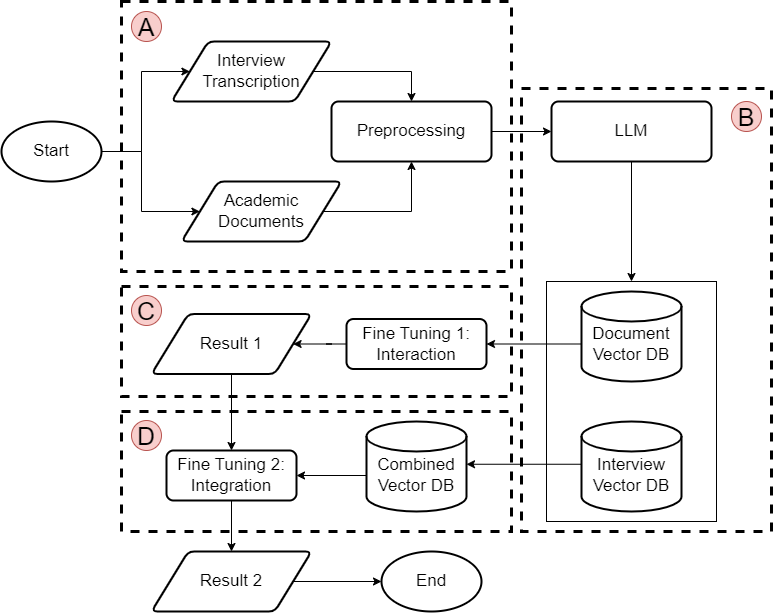
\includegraphics[scale=0.3]{eng-main.png}}
    \caption{System Flowchart}
    \label{fig:main-flowchart}
\end{figure}

The flow of this process is illustrated in Figure \ref{fig:main-flowchart}. The process broadly starts with reading and collecting data from interviews and documents, followed by a preprocessing step to prepare the data. The next step involves a LLMs to understand the content and generate a vector representation of the collected information. 

Then, the vector representation is then stored into a Vector Database (Vector DB) which will be the source of knowledge. The system involves two stages of fine-tuning, first process begins with documents only, where the system extracts relevant information from academic documents and generates \textbf{Result 1}, an answer based solely on the document dataset. In the second stage, the system combines information from multiple sources, such as interviews and documents, during a broader fine-tuning process. This produces \textbf{Result 2}, an answer generated by integrating knowledge from both documents and interviews, offering more comprehensive and contextualized responses. \\
\\
\textbf{\textit{Data Preprocessing}} The pre-processing stage is a critical initial step in preparing optimal input for the LLMs. Figure \ref{fig:preprocessing} illustrates the data pre-processing flow that will be conducted. This process consists of two main parts: pre-processing of document data and pre-processing of interview data.

\begin{figure}[htbp]
        \centerline{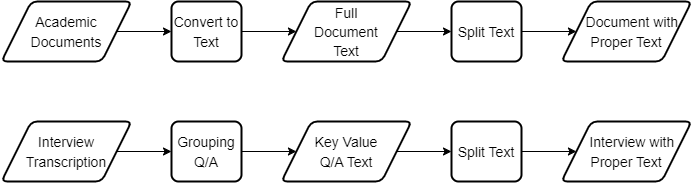
\includegraphics[scale=0.4]{eng-preproc.png}}
        \caption{Data Preprocessing}
        \label{fig:preprocessing}
    \end{figure}
    
\begin{enumerate}
    \item \textbf{Pre-Processing Document Data}
    Initially, data from academic documents, typically in PDF format, undergoes conversion from PDF to text using the LangChain framework's document loader. Specifically, we use the \textbf{PyPDFLoader} from \textbf{document\_loaders} in LangChain to perform this conversion. This step ensures that the text is in a format that can be processed by the LLM. After conversion, the text from the documents is segmented by sentences, enabling the LLMs to understand the content more deeply by considering sentence structure. This segmentation is crucial to ensure that information from the documents can be effectively accessed and comprehended by the model.
    
    \item \textbf{Pre-Processing Interview Data} For interview data, automatic transcription is performed using the \textbf{YouTubeLoader} library from LangChain's  \textbf{document\_loaders}. This library facilitates the automatic extraction and transcription of audio from interviews. The initial step involves grouping questions and answers into related entities, allowing the model to comprehensively understand the context of the discussions. Following this, the pre-processing of interview data mirrors that of document data, with text segmentation by sentences. This creates a uniform data structure, facilitating the model's understanding of information extracted from interviews.
\end{enumerate}

Through meticulous and careful pre-processing, the data is expected to provide a better and more contextual representation when presented to the LLMs. This process serves as a crucial initial step in building a reliable and effective KAS in the academic environment. \\
\\
\textbf{\textit{LLM}} The next stage after data pre-processing is knowledge extraction using the LLMs.

\begin{algorithm}
    \caption{Tokenization, Embedding, and Vector Storage}
    \begin{algorithmic}[1]
    \State \textbf{Input:} text data $T$, LLM model $M$, vector database $VDB$
    \State \textbf{Output:} vector database updated with embeddings
    
    \State /* Tokenize the input text */
    \State tokens $\gets$ tokenize($T$, $M$)
    
    \State /* Generate embeddings for each token */
    \State embeddings $\gets$ []
    \ForAll{token $\in$ tokens}
        \State embedding $\gets M.embed(token)$
        \State append(embedding, embeddings)
    \EndFor
    
    \State /* Store embeddings in vector database */
    \ForAll{embedding $\in$ embeddings}
        \State store($VDB$, embedding)
    \EndFor
    
    \State \Return $VDB$
    \end{algorithmic}
\end{algorithm}

This process includes several critical steps outlined as follows:

\begin{enumerate}  
    \item \textbf{Tokenization} After reading the text, tokenization is performed to break the text into tokens or smaller units that can be processed by the model. Tokenization helps the model to understand the structure and meaning of words within the context of sentences.
    
    \item \textbf{Embedding} The embedding process involves representing words as numerical vectors. Each word in the text is transformed into a vector that captures the word's meaning. This process allows the model to work with continuous representations and to understand semantic relationships between words.
    
    \item \textbf{Storing in Vector Database} The vectors generated from the embedding process are stored in a Vector Database (Vector DB). The Vector DB acts as a repository for the vector representations of the processed documents and interviews. This stored data serves as the knowledge base that can be accessed in subsequent stages.
\end{enumerate}

By using the LLMs, the system can understand and represent the information extracted from documents and interviews more effectively. These steps connect the understanding of text with vector representations that the system can access and process in later stages.\\ 
\\
\textbf{\textit{Fine Tuning}} Fine-tuning is a critical stage in optimizing the model to respond more accurately and relevantly to specific questions or contexts. We divided the fine tuning into two subprocesses: first at the individual level using a single Vector Database (Vector DB), and second at the aggregation level using a combined vector database.

\begin{figure}[htbp]
    \centerline{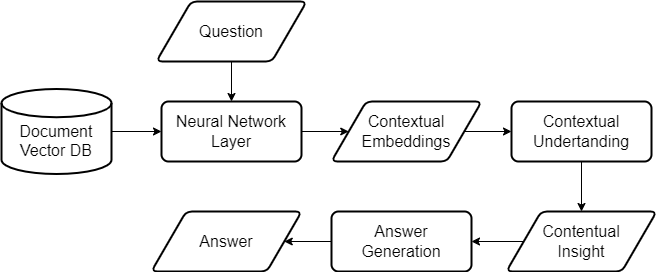
\includegraphics[scale=0.4]{eng-fine1.png}}
    \caption{Fine Tuning}
    \label{fig:fine-tuning-1}
\end{figure}

\begin{enumerate}
    \item \textbf{Fine Tuning \#1} The first fine-tuning phase, shown in Figure \ref{fig:fine-tuning-1}, begins by using vectors from a Vector Database as input. Neural Network layers, or embeddings, are used to fine-tune the model, improving its ability to understand content contextually. "Contextual" refers to capturing multiple meanings and synonyms. After this, the model enters a Contextual Understanding phase, interpreting queries better through GPT. Finally, the model uses similarity search during Answer Generation to provide the most relevant responses based on refined vector representations.
                    
    \item \textbf{Fine Tuning \#2} Involves a similar process but at the aggregation level using the combined vector database. In this stage, vector representations from various sources of information are integrated, and the model undergoes another round of fine-tuning. The focus here is on understanding and responding to questions or contexts that involve multiple aspects of knowledge acquisition.
\end{enumerate}

Through these two stages of fine-tuning, it is anticipated that the model will deliver improved knowledge acquisition results, taking into account the depth of information from the involved sources and generating more contextual and relevant responses.

\section{System Demonstration and Practical Use}
\subsection{Tools and Technologies Used}
The development and functionality of the system are powered by several key technologies:
\begin{itemize}
    \item Streamlit: Used for the front-end interface of the web-based chatbot, enabling users to interact with the system in a user-friendly manner.
    \item LangChain: A critical framework used to integrate different language models, such as GPT, and manage workflows for document processing and question answering.
    \item FAISS Vector Store: Used for storing and retrieving vectorized embeddings of the knowledge processed from the input data. This ensures efficient and accurate search capabilities within the knowledge base.
    \item OpenAI Embedding and Chat: The core LLMs and embedding generation tool. OpenAI's GPT is used to generate embeddings, process user inputs, and provide accurate, context-based responses.
\end{itemize}

\subsection{Input Page: Data Upload and Processing}
This section of the system allows users to upload various types of data to be processed and added to the knowledge base. Users can submit different data formats to capture knowledge in diverse ways:
\begin{itemize}
    \item PDF Files: Users can upload academic documents, research papers, or administrative files, which are processed using LangChain's PyPDFLoader. The system extracts the text and converts it into a structured format.
    \item JSON Files: Structured data in JSON format can be directly uploaded, allowing the system to quickly process datasets or academic records.
    \item YouTube URLs: Leveraging LangChain's YouTubeLoader, users can input a YouTube URL for automatic transcription. The system extracts the text from the video's captions and processes it for further use.
    \item Raw Text: Users can input plain text directly, making the system flexible for adding knowledge from various informal sources like interviews, lectures, or meeting notes.
\end{itemize}

Once the input data is uploaded, the system processes and converts it into embeddings using OpenAI's embedding model. The vectorized data is stored in the FAISS Vector Store for quick and contextually relevant retrieval.

\subsection{Chatbot Page: Interactive Knowledge Access}
The chatbot interface allows users to interact directly with the knowledge stored in the system:
\begin{itemize}
    \item \textbf{Interaction with Knowledge}: Users can ask questions related to the data that has been processed and stored in the vector database. The chatbot leverages GPT to understand the questions, retrieve relevant information from the embeddings, and generate contextual answers.
    \item \textbf{Memory Scenario}: The chatbot incorporates a memory scenario where session-specific data is stored temporarily. This allows the chatbot to maintain a context-aware conversation within a session, enabling it to remember past questions and answers. However, this session memory is cleared once the session ends, ensuring privacy and a fresh start for future interactions.
\end{itemize}

For example: \\
\textbf{User's Question}: \textit{``What should be considered in the Final Project revision process?''} \\

\textbf{Chatbot Response}: \\
In the Final Project revision process, the following points must be considered:
\begin{enumerate}
    \item Students are given a maximum of 15 calendar days to complete the revision after the results of the Final Project hearing are decided.
    \item If the revision is not completed within 15 days, the Final Project index value will drop by one level.
    \item If the revision is not completed within 30 days, the student is declared to have failed.
    \item The results of the revision must be validated by the Supervisor before being submitted to the LAAK admin for the Judicial Hearing process.
\end{enumerate}


\section{Evaluation}
To obtain a comprehensive and optimal evaluation of the KAS, we use three primary evaluation metrics: ROUGE Score, BERT Score, and manual evaluation. Combining these three methods allows for a thorough assessment of the quality of answers generated by the system.

\subsection{ROUGE Score}
This metric provides insight into the surface-level text similarity, such as words and phrases, between the generated summaries and reference texts \cite{Lin2004}. It helps assess how well the generated summaries match the reference texts considered as gold standard.
\begin{itemize}
    \item \textbf{Precision}: Precision is calculated using the formula:
    \[
    \text{Precision (P)} = \frac{\text{TP}}{\text{TP + FP}}
    \]
    where:
    \begin{itemize}
        \item TP (True Positives): The number of overlapping n-grams between the generated results and the reference. In the context of ROUGE-N, this includes n-grams appearing in both the generated result and the reference text.
        \item TP+FP (Total Predicted Positives): The total number of n-grams in the generated results. This includes both correctly and incorrectly predicted n-grams.
    \end{itemize}
    A higher precision value indicates that the generated results are more accurate and aligned with the reference content.

    \item \textbf{Recall}: Recall is calculated using the formula:
    \[
    \text{Recall (R)} = \frac{\text{TP}}{\text{TP + FN}}
    \]
    where:
    \begin{itemize}
        \item TP (True Positives): The number of overlapping n-grams between the generated results and the reference.
        \item TP+FN (Total Actual Positives): The total number of n-grams in the reference text. This includes all n-grams that should have been generated based on the reference.
    \end{itemize}
    Recall provides insight into how well the predictions capture the information present in the reference. A high recall value indicates that the predictions cover most of the relevant information from the reference.

    \item \textbf{\( F_{1}\text{-score} \)}: 
    \( F_{1}\text{-score} \) is calculated using the formula:
    \[
    F_{1}\text{-score} = 2 \times \left( \frac{\text{Precision} \times \text{Recall}}{\text{Precision} + \text{Recall}} \right)
    \]
    \( F_{1}\text{-score} \) combines precision and recall into a single metric that provides a holistic view of the summary quality. A higher \( F_{1}\text{-score} \) indicates a better balance between precision and recall.
\end{itemize}
    
\subsection{BERT Score}
BERT Score evaluates semantic similarity between the generated text and reference text using contextual embeddings from the BERT model \cite{Zhang2020}.
\begin{itemize}
    \item \textbf{Precision}: Precision is calculated using the formula:
    \[
    \text{Precision} (P) = \frac{1}{|G|} \sum_{w \in G} \max_{w' \in R} \text{sim}(w, w')
    \]
    where:
    \begin{itemize}
      \item \( G \) is the set of words in the generated text.
      \item \( R \) is the set of words in the reference text.
      \item \( \text{sim}(w, w') \) is the cosine similarity between the embeddings of words \( w \) and \( w' \).
    \end{itemize}

    \item \textbf{Recall}: Recall is calculated using the formula:
    \[
    \text{Recall} (R) = \frac{1}{|R|} \sum_{w \in R} \max_{w' \in G} \text{sim}(w, w')
    \]
    where:
    \begin{itemize}
      \item \( R \) is the set of words in the reference text.
      \item \( G \) is the set of words in the generated text.
      \item \( \text{sim}(w, w') \) is the cosine similarity between the embeddings of words \( w \) and \( w' \).
    \end{itemize}

    \item \textbf{\( F_{1}\text{-score} \)}: 
    \( F_{1}\text{-score} \) is calculated using the formula:
    \[
    F_{1}\text{-score} = 2 \times \left( \frac{\text{Precision} \times \text{Recall}}{\text{Precision} + \text{Recall}} \right)
    \]
\end{itemize}
    
\subsection{Manual Evaluation}
Manual evaluation involved two experts with over  25 years of experience in their respective fields, including a program secretary who is deeply familiar with academic processes and tacit knowledge within the institution. They evaluated responses based on contextual relevance. Questions spanned six distinct topics, with 10 questions per topic. Each answer was rated on a relevance scale, ranging from "not relevant" to "highly relevant." This approach provided detailed insights into how well the system handled context and generated accurate, institutionally aligned answers, offering a deeper assessment than automated metrics like ROUGE Score and BERT Score.

\subsection{Results}
Combining these three approaches ensures a comprehensive assessment of the KAS, considering both surface-level text similarity and semantic similarity, and provides a fuller picture of the quality of the answers produced by the system.

For more detailed information, the model performance results with ROUGE Score can be seen in Table \ref{tab:rouge-bert-table}. The table shows that scoring using unigrams dominates, with precision as the highest metric.

\begin{table}[htbp]
    \centering
    \caption{Rouge and BERT Scores}
    \setlength{\arrayrulewidth}{0.5pt} % Adjust the thickness of vertical lines
    \renewcommand{\arraystretch}{1.5} % Adjust vertical spacing
    \begin{tabular}{|c|c|c|c|c|c|c|c|c|c|}
        \cline{2-10}
        \multicolumn{1}{c|}{} & \multicolumn{3}{c|}{\textbf{Unigram (Rouge)}} & \multicolumn{3}{c|}{\textbf{Bigram (Rouge)}} & \multicolumn{3}{c|}{\textbf{BERT Score}} \\ 
        \hline
        \textbf{Dataset} & \textbf{PREC} & \textbf{REC} & \textbf{F1} & \textbf{PREC} & \textbf{REC} & \textbf{F1} & \textbf{PREC} & \textbf{REC} & \textbf{F1} \\
        \hline
        Document & \textbf{0.72} & 0.12 & 0.20 & 0.38 & 0.04 & 0.09 & \textbf{0.74} & 0.58 & 0.65 \\ 
        \hline
        Interview & \textbf{0.79} & 0.11 & 0.19 & 0.40 & 0.03 & 0.06 & \textbf{0.76} & 0.60 & 0.67 \\ 
        \hline
        Combined & \textbf{0.74} & 0.13 & 0.21 & 0.40 & 0.05 & 0.09 & \textbf{0.75} & 0.59 & 0.66 \\ 
        \hline
    \end{tabular}
    \label{tab:rouge-bert-table}
\end{table}

For the model performance results with BERT Score can be seen in Table  \ref{tab:rouge-bert-table}. The table shows that the model performs well contextually, with the highest score still obtained in the precision metric. A high precision score indicates that the model tends to produce answers that are highly relevant and semantically in line with the existing references.

However, the combined dataset scored lower than the interview dataset due to the PDF-to-text extraction in documents. This extraction method has weaknesses that affect the quality of the text, leading to a lower combined result. Therefore, even though the precision score is high, it is important to consider recall and F1 score metrics. A lower recall score may indicate that the model missed some relevant information, and the F1 score balances precision and recall, highlighting areas for improvement.

Then, for the manual evaluation results, the evaluators were two individuals who provided the tacit knowledge for the system: an academic secretary and a senior lecturer. Their role was crucial as they had firsthand experience with the implicit knowledge encoded into the system, enabling them to assess the relevance of the system's responses accurately.

The evaluation results are as follows:the following results were obtained: \\
Out of a total of 60 questions:
\begin{itemize}
    \item \textbf{86}\% of the answers were rated as \textbf{highly relevant} with a score of 3.5 - 5
    \item \textbf{2}\% of the answers were rated \textbf{moderately relevant} with a score of 3
    \item and only \textbf{12}\% of the answers were rated \textbf{less relevant} with a score of 1-2.5
\end{itemize}

These results show that the system performs quite well in answering questions in a relevant and contextual manner according to expert judgment.

Thus, the use of the ROUGE metric as a guide for quantitative evaluation, then the BERT metric for semantic evaluation and together with the input from the expert evaluation, can provide a more holistic and detailed understanding of the overall quality of the developed text generation system.

\section{Conclusion}
In this research, a system for automatic knowledge acquisition in the academic domain has been successfully proposed and implemented using LLMs and fine-tuning techniques. The evaluation conducted shows that the system is capable of acquiring, understanding, and responding to various types of questions and contexts related to the academic environment.

The precision of knowledge acquisition, measured by comparison with information provided by experts in interviews, demonstrates positive results. The responses generated by the system also show a good level of contextuality, with the ability to respond accurately to questions referring to information from academic documents and interview results.

However, there are areas that can be improved. Analyzing the system's speed and efficiency could be a focus for further development to ensure responsiveness in a dynamic academic environment.

Overall, the system has shown good precision, particularly in tests using questions that align with the existing documents. However, to further enhance performance, improvements in both data and system development are needed. Thus, these improvement steps will be an integral part of future development to ensure the success and reliability of the KAS in the academic environment.


%
% ---- Bibliography ----
%
% BibTeX users should specify bibliography style 'splncs04'.
% References will then be sorted and formatted in the correct style.
%
\bibliographystyle{splncs04}
\bibliography{references}
%
\end{document}
